
%(BEGIN_QUESTION)
% Copyright 2009, Tony R. Kuphaldt, released under the Creative Commons Attribution License (v 1.0)
% This means you may do almost anything with this work of mine, so long as you give me proper credit

Determine whether or not the following faults (considered individually) could account for this air pressure regulating system failing with zero pressure in the receiver vessel.  Answer either ``yes'' or ``no'' for each fault:

$$\includegraphics[width=15.5cm]{i03848x01.eps}$$

$$\includegraphics[width=15.5cm]{i03848x02.eps}$$

\begin{itemize}
\item{} Receiver vessel drain valve left open
\item{} Transmitter block valve shut and bleed valve open
\item{} Transmitter block valve open and bleed valve shut
\item{} PIC left in manual mode, 100\% output (20 mA to I/P)
\item{} Cable PV-6 severed (failed open)
\item{} I/P air supply shut off
\item{} Short between TB-52, terminals 1 and 2
\item{} Short between TB-52, terminals 15 and 16 
\item{} PT-6 miscalibrated, registering 5 PSI too high
\item{} PY-6 output failed high (15 PSI) 

\end{itemize}

\underbar{file i03848}
%(END_QUESTION)





%(BEGIN_ANSWER)

\begin{itemize}
\item{} Receiver vessel drain valve left open -- {\bf No}
\item{} Transmitter block valve shut and bleed valve open -- {\bf No}
\item{} Transmitter block valve open and bleed valve shut -- {\bf No}
\item{} PIC left in manual mode, 100\% output (20 mA to I/P) -- {\bf Yes}
\item{} Cable PV-6 severed (failed open) -- {\bf No}
\item{} I/P air supply shut off -- {\bf No}
\item{} Short between TB-52, terminals 1 and 2 -- {\bf Yes}
\item{} Short between TB-52, terminals 15 and 16 -- {\bf No}
\item{} PT-6 miscalibrated, registering 5 PSI too high -- {\bf No}
\item{} PY-6 output failed high (15 PSI) -- {\bf Yes}
\end{itemize}


%(END_ANSWER)





%(BEGIN_NOTES)

\vskip 20pt \vbox{\hrule \hbox{\strut \vrule{} {\bf Virtual Troubleshooting} \vrule} \hrule}

This question is a good candidate for a ``Virtual Troubleshooting'' exercise.  Presenting the diagram to students, you first imagine in your own mind a particular fault in the system.  Then, you present one or more symptoms of that fault (something noticeable by an operator or other user of the system).  Students then propose various diagnostic tests to perform on this system to identify the nature and location of the fault, as though they were technicians trying to troubleshoot the problem.  Your job is to tell them what the result(s) would be for each of the proposed diagnostic tests, documenting those results where all the students can see.

During and after the exercise, it is good to ask students follow-up questions such as:

\begin{itemize}
\item{} What does the result of the last diagnostic test tell you about the fault?
\item{} Suppose the results of the last diagnostic test were different.  What then would that result tell you about the fault?
\item{} Is the last diagnostic test the best one we could do?
\item{} What would be the ideal order of tests, to diagnose the problem in as few steps as possible?
\end{itemize}


%INDEX% Basics, control loop troubleshooting

%(END_NOTES)


